\documentclass{article}

\usepackage[]{xrcise}

\subject{Informationsgestützte Modellierung von Organisationen}
\semester{Summer 2024}
\author{Leopold Lemmermann}

\begin{document}\createtitle

\sheet{Vorlesungsfragen}
\begin{exercise}{Einführung}
  \begin{enumerate}
    \item Was ist ein Modell?
          \begin{solution}
            Ein Modell ist eine vereinfachte Darstellung eines realen oder theoretischen Systems, die wesentliche Merkmale dieses Systems erfasst, um es besser verstehen und analysieren zu können.
          \end{solution}

    \item Welche typischen Eigenschaften weisen Modelle auf?
          \begin{solution}
            Modelle sind typischerweise abstrakt, vereinfacht, formalisiert und perspektivisch. Das bedeutet, sie abstrahieren von unwesentlichen Details, vereinfachen komplexe Zusammenhänge, folgen bestimmten formalen Regeln oder mathematischen Strukturen und betrachten das System aus einer bestimmten Perspektive.
          \end{solution}

    \item Zu welchen Zwecken werden Modelle gebildet?
          \begin{solution}
            Modelle werden gebildet, um komplexe Sachverhalte zu verstehen, zu analysieren, zu beschreiben, zu prognostizieren, zu simulieren, zu optimieren oder Entscheidungen zu unterstützen.
          \end{solution}

    \item Nennen Sie jeweils ein Beispiel für Komplexitätsreduzierung durch Idealisierung und durch Abstraktion.
          \begin{solution}
            Idealisierung reduziert Komplexität durch Annahmen wie den Homo Oeconomicus. Abstraktion reduziert Komplexität durch die Betrachtung einer Fabrik als eine Einheit.
          \end{solution}

    \item Worin unterscheiden sich Simulationsmodelle und analytische Modelle? Geben Sie zwei Merkmale an.
          \begin{solution}
            Methoden (numerisch+stochastisch v. mathematisch+logisch): Simulationsmodelle verwenden numerische und stochastische Methoden zur Modellierung, während analytische Modelle auf mathematischen und logischen Ansätzen basieren.
            Flexibilität (anpassbar v. spezifische Annahmen): Simulationsmodelle sind flexibel und anpassbar an verschiedene Szenarien, während analytische Modelle spezifische mathematische Annahmen verwenden und weniger flexibel sind.
          \end{solution}

    \item Worin unterscheiden sich Simulationen mit wissenschaftlichem Anspruch und Computerspiele des Genres "Simulation"? Nennen Sie zwei Merkmale.
          \begin{solution}
            Wissenschaftliche Simulationen durchlaufen strenge Validierungsprozesse und sind reproduzierbar, um die Genauigkeit ihrer Ergebnisse sicherzustellen. Computerspiele des Genres "Simulation" sind hingegen weniger auf wissenschaftliche Genauigkeit ausgerichtet und legen mehr Wert auf Unterhaltung und Benutzererlebnis.
          \end{solution}
  \end{enumerate}
\end{exercise}

\begin{exercise}{Diskrete Modellierung}
  \begin{enumerate}
    \item Beschreiben Sie das grundsätzliche Ablaufschema der ereignisdiskreten Simulation!
          \begin{solution}
            Das grundsätzliche Ablaufschema der ereignisdiskreten Simulation umfasst die Initialisierung, die Ereignisverarbeitung, die Zustandsaktualisierung und die Terminierung.
          \end{solution}

    \item Welche typischen Abbruchbedingungen gibt es in der ereignisdiskreten Simulation?
          \begin{solution}
            Simulationsläufe werden beendet durch Zeitbedingungen (z.B. wenn eine bestimmte Simulationszeit erreicht ist), Ereignisbedingungen (z.B. wenn eine bestimmte Anzahl von Kunden erreicht ist) oder Ressourcenbedingungen (z.B. wenn keine Ressourcen mehr verfügbar sind).
          \end{solution}

    \item Beschreiben Sie das grundsätzliche Vorgehen zum Entwurf eines prozessorientierten Simulationsmodells!
          \begin{solution}
            Beim Entwurf eines prozessorientierten Simulationsmodells identifiziert man relevante Systemobjekte, fügt Attribute hinzu, arbeitet Aktivitäten aus, definiert Lebenszyklen der Entitäten, legt Beziehungen zwischen den Entitäten fest, identifiziert Ereignisse und ordnet Überschneidungsbereiche zu.
          \end{solution}

    \item Vergleichen Sie ereignis- und prozessorientierte Modellierung! Stellen Sie insbesondere wesentliche Unterschiede dar!
          \begin{solution}
            Der Hauptunterschied liegt darin, dass ereignisorientierte Modelle auf diskreten Ereignissen basieren und zeitgesteuert sind, während prozessorientierte Modelle den Fokus auf den Ablauf von Aktivitäten und Prozessen legen, die intern verwaltet werden.
          \end{solution}

    \item Begründen Sie, warum für Lagerhaltungsmodelle typischerweise der ereignisorientierte Modellierungsstil besser geeignet ist als der prozessorientierte Modellierungsstil.
          \begin{solution}
            Der ereignisorientierte Modellierungsstil ist besser geeignet, da Lagerhaltungsmodelle stark von diskreten Ereignissen wie Bestellungen und Lieferungen abhängen, deren Zeitpunkt und Auftreten nicht direkt von internen Prozessen abhängt.
          \end{solution}

    \item Wie modelliert man wiederholte Ankünfte…
          \begin{enumerate}
            \item …im ereignisorientierten Ansatz?
                  \begin{solution}
                    Im ereignisorientierten Ansatz werden wiederholte Ankünfte durch ein regelmäßig auftretendes Ankunftsereignis modelliert.
                  \end{solution}

            \item …im prozessorientierten Ansatz?
                  \begin{solution}
                    Im prozessorientierten Ansatz werden wiederholte Ankünfte durch Timer-/Nachrichten-Startereignisse modelliert.
                  \end{solution}
          \end{enumerate}

    \item Skizzieren Sie das BPMN-Prozessdiagramm eines typischen Kunden-Prozesses z.B. Job im Produktionssystem.
          \begin{solution}
            Ein BPMN-Prozessdiagramm eines typischen Kunden-Prozesses könnte Start- und Endereignisse, Aktivitäten, Entscheidungen, Verzweigungen und Zusammenführungen umfassen.
          \end{solution}

    \item Nennen Sie drei typischerweise in der Simulation verwandte Typen von BPMN-Zwischenereignissen und beschreiben Sie ihre Semantik.
          \begin{solution}
            Typische BPMN-Zwischenereignisse sind Timer-Ereignisse, Signal-Ereignisse, Nachrichten-Ereignisse.
          \end{solution}

    \item Warum sind für die BPMN-Prozesssimulation implizit erzeugte Warteschlangen notwendig?
          \begin{solution}
            Implizit erzeugte Warteschlangen sind notwendig, um die Reihenfolge der Aktivitäten in einem Prozess zu steuern und Engpässe im Ablauf zu identifizieren.
          \end{solution}

    \item Wie kann man in BPMN-Prozessdiagrammen die begrenzte Wartebereitschaft eines Kunden abbilden?
          \begin{solution}
            Das kann durch ein Timer-Boundary-Event modelliert werden. Hierbei wird das Timer-Event an die Aktivität angehängt und von dort ein weiterer Pfad gestartet.
          \end{solution}
  \end{enumerate}
\end{exercise}

\begin{exercise}{Simulationssoftware}
  \begin{enumerate}
    \item Welche Arten von Simulationssoftware kann man unterscheiden?
          \begin{solution}
            Man kann Simulationssoftware in allgemeine Programmiersprachen, Simulationssoftware auf Werkzeugebene (generelle Simulationssoftware) und spezialisierte Simulationssoftware unterteilen.
          \end{solution}

    \item Nennen Sie jeweils zwei Vor- und Nachteile von Simulationssoftware auf Werkzeugebene.
          \begin{solution}
            Vorteile: Einfache Bedienung, schnelle Modellerstellung. Nachteile: Eingeschränkte Flexibilität bei komplexen Modellen, geringere Leistungsfähigkeit im Vergleich zu spezialisierten Lösungen.
          \end{solution}

    \item Welche simulationsspezifischen Auswahlkriterien für Simulationssoftware kennen Sie?
          \begin{solution}
            Auswahlkriterien sind z.B. Kosten, Funktionsumfang, Benutzerfreundlichkeit, Skalierbarkeit und Dokumentation.
          \end{solution}

    \item Beschreiben Sie Potential und Grenzen von Animation in der Simulation.
          \begin{solution}
            Animationen können helfen, komplexe Prozesse zu veranschaulichen und das Verständnis zu fördern. Jedoch können sie auch ablenken und die eigentliche Analyse der Simulation beeinträchtigen.
          \end{solution}

    \item Beschreiben Sie den Zusammenhang zwischen konzeptuellem Modell \& Computermodell einer Simulationsstudie mit IYOPRO.
          \begin{solution}
            Das konzeptuelle Modell beschreibt abstrakt das zu untersuchende System. Das Computermodell in IYOPRO ist die Implementierung dieses konzeptionellen Modells, das zur Durchführung der Simulation verwendet wird.
          \end{solution}

    \item Inwiefern unterstützt IYOPRO die Modellierung und Simulation von Ressourcen?
          \begin{solution}
            IYOPRO unterstützt die Modellierung und Simulation von Ressourcen durch die Definition von Ressourcen mit Rollen, welche von Aktivitäten verwendet werden können.
          \end{solution}

    \item Gehen Sie insbesondere auf die möglichen Zustände einer Ressource ein.
          \begin{solution}
            Mögliche Zustände einer Ressource in IYOPRO können sein: Idle (verfügbar für Nutzung), In use (aktuell in Nutzung), Waiting (Von Prozess gefordert aber noch nicht verwendet, da andere Ressourcen nicht verfügbar) oder setup/post-processing.
          \end{solution}

    \item Worin unterscheiden sich Blackbox- und Whitebox-Komponenten in Software-Frameworks? Nennen Sie jeweils ein Beispiel in DESMO-J!
          \begin{solution}
            Blackbox-Komponenten in DESMO-J sind zum Beispiel die Simulationsinfrastruktur. Diese ist nicht direkt zugänglich. Whitebox-Kompoenten sind die abstrakten Klassen (Hot Spots) für das Modell. Diese müssen um Modelldetails erweitert werden.
          \end{solution}
  \end{enumerate}
\end{exercise}

\begin{exercise}{Simulationsstatistik \& Optimierung}
  \begin{enumerate}
    \item Warum sollte man Simulationsläufe mehrfach wiederholen?

          \begin{solution}
            Simulationsläufe werden mehrfach wiederholt, um Zufallseinflüsse zu reduzieren und die Aussagekraft der Ergebnisse zu verbessern. Dadurch können robustere Schlussfolgerungen gezogen werden.
          \end{solution}

    \item Wie kann man Pseudozufallszahlen erzeugen, die im Intervall [0,1) näherungsweise stetig gleichverteilt sind?

          \begin{solution}
            Pseudozufallszahlen, die näherungsweise stetig gleichverteilt sind, können mit Generatoren wie dem linearen Kongruenzgenerator oder dem Mersenne-Twister erzeugt werden. Diese Generatoren erzeugen Zahlen, die statistischen Tests für Gleichverteilung standhalten.
          \end{solution}

    \item Was versteht man unter einem Konfidenzintervall?

          \begin{solution}
            Ein Konfidenzintervall ist ein Intervall, innerhalb dessen ein Schätzwert einer Messgröße mit einer bestimmten Wahrscheinlichkeit (z.B. 95\%) liegt. Es dient dazu, die Genauigkeit und Zuverlässigkeit von Schätzungen zu quantifizieren.
          \end{solution}

    \item Welche Bestandteile gehören zu einem Optimierungsproblem?

          \begin{solution}
            Ein Optimierungsproblem umfasst typischerweise eine Zielfunktion, die maximiert oder minimiert werden soll, Entscheidungsvariablen, die optimiert werden können, und Nebenbedingungen, die die zulässigen Lösungen einschränken.
          \end{solution}

    \item Erläutern Sie die grundsätzliche Vorgehensweise eines genetischen Algorithmus!

          \begin{solution}
            Der genetische Algorithmus beginnt mit einer zufälligen Population von Lösungskandidaten. Diese werden iterativ durch Selektion, Rekombination (Crossover), Mutation, Evaluation und Ersetzung verbessert, wobei jeweils die besten Lösungen ausgewählt werden, um die nächste Generation zu bilden.
          \end{solution}
  \end{enumerate}
\end{exercise}

\begin{exercise}{Simulationspraxis}
  \begin{enumerate}
    \item "Wir müssen unsere Logistik verbessern!" - Welche Ziele versteht man hierunter üblicherweise in Unternehmen?

          \begin{solution}
            Typische Ziele sind die Senkung der Betriebskosten, die Steigerung der Effizienz in der Logistikabwicklung und die Reduzierung der Lieferzeiten.
          \end{solution}

    \item Was spricht für die Beauftragung externer Simulationsdienstleister, um eine betriebliche Simulationsstudie durchzuführen? Was spricht dagegen? Nennen Sie jeweils zwei Faktoren!

          \begin{solution}
            Pro: Externe Simulationsdienstleister bieten oft spezialisiertes Wissen und eine unvoreingenommene Perspektive. Contra: Die Kosten können hoch sein, und externe Dienstleister verfügen möglicherweise nicht über das detaillierte betriebliche Wissen, das für eine präzise Modellierung erforderlich ist.
          \end{solution}

    \item Welche Rollen kann man bei der Durchführung einer Simulationsstudie unterscheiden?

          \begin{solution}
            Zu den Rollen gehören der Auftraggeber, der Projektleiter, der Simulationsdienstleister und die Anwender, die die Ergebnisse interpretieren und darauf reagieren.
          \end{solution}

    \item Nennen Sie drei typische Fehlerquellen in einer Simulationsstudie!

          \begin{solution}
            Häufige Fehlerquellen sind falsche Annahmen über das Systemverhalten, Modellierungsfehler, die die Realitätsnähe beeinträchtigen, und Implementierungsfehler, die falsche oder fehlerhafte Modelle ausführen lassen.
          \end{solution}
  \end{enumerate}
\end{exercise}

\begin{exercise}{(IT-)Organisation \& Prozesse}
  \begin{enumerate}
    \item Setzen Sie Porters Wertschöpfungskette in Beziehung zu den beschriebenen Unternehmensaktivitäten!
          \begin{solution}
            Die Porters Wertschöpfungskette unterteilt Unternehmensaktivitäten in primäre (wie Eingangslogistik, Produktion, Marketing und Vertrieb, Service) und unterstützende Aktivitäten (wie Beschaffung, Technologieentwicklung, Personalmanagement, Infrastruktur). Diese Aktivitäten sind direkt mit der Wertschöpfung verbunden und helfen dabei, strategische Vorteile zu schaffen und zu erhalten.
          \end{solution}

    \item Erklären Sie Sinn und Zweck von Modellierung und leiten Sie daraus Vor- und Nachteile des modellbasierten Problemlösens ab!
          \begin{solution}
            Modellierung dient dazu, komplexe Systeme zu vereinfachen, zu verstehen und zu analysieren. Vorteile sind unter anderem die strukturierte Herangehensweise an Probleme, die Möglichkeit der Vorhersage und Simulation sowie die Veranschaulichung von Zusammenhängen. Nachteile können Abstraktionen sein, die möglicherweise wichtige Details vernachlässigen, sowie der Aufwand für die Erstellung und Pflege komplexer Modelle.
          \end{solution}

    \item Modellieren Sie einen gegebenen Geschäftsprozess und schätzen Sie die Performanz eines Prozesses anhand qualitativer sowie quantitativer Analyseverfahren ab!
          \begin{solution}
            Die Modellierung eines Geschäftsprozesses kann mittels BPMN-Diagrammen erfolgen. Qualitative Analysen umfassen Aspekte wie Benutzerfreundlichkeit und Flexibilität, während quantitative Analysen Metriken wie Durchlaufzeiten und Ressourcenverbrauch messen können. Dies ermöglicht eine ganzheitliche Bewertung der Prozessperformance.
          \end{solution}

    \item Beschreiben Sie Methoden und Strategien des Komplexitätsmanagements!
          \begin{solution}
            Methoden des Komplexitätsmanagements umfassen z.B. die Modularisierung von Systemen, die Standardisierung von Prozessen und die Reduktion von Schnittstellen. Strategien beinhalten die Förderung von Transparenz, die Anpassung der Organisationsstruktur an Komplexitätsanforderungen und die Verwendung von IT-gestützten Werkzeugen zur Komplexitätsbewältigung.
          \end{solution}

    \item Erklären Sie, weshalb es so vielfältige Aufbauten von Organisationen gibt und verstehen Sie, welche Faktoren einen Einfluss auf das Design von Organisationen haben!
          \begin{solution}
            Die Vielfalt der Organisationsformen resultiert aus unterschiedlichen Geschäftsmodellen, Branchenanforderungen, Marktbedingungen und kulturellen Einflüssen. Faktoren wie Größe, Strategie, Technologieeinsatz und globaler Wettbewerb beeinflussen das Design von Organisationen maßgeblich.
          \end{solution}

    \item Erklären Sie den Sinn und Zweck der Referenzmodellierung und leiten Sie daraus Vor- und Nachteile ab!
          \begin{solution}
            Referenzmodellierung dient dazu, bewährte Praktiken und Standards in Form von Modellen bereitzustellen, die als Grundlage für die Gestaltung und Implementierung von Geschäftsprozessen dienen. Vorteile sind die Beschleunigung von Implementierungszeiten und die Förderung von Konsistenz. Nachteile könnten Beschränkungen bei der Anpassung an spezifische Anforderungen sein.
          \end{solution}

    \item Welches sind verschiedene Koordinationsmechanismen in Organisationen und wie können diese in unterschiedlichen Aufbauten von Organisationen realisiert werden?
          \begin{solution}
            Koordinationsmechanismen umfassen hierarchische Steuerung, Marktmechanismen, bürokratische Regelungen und informelle Netzwerke. Diese können je nach Organisationsstruktur und -kultur unterschiedlich ausgeprägt sein, z.B. stark hierarchisch in traditionellen Organisationen oder eher durch flexible Netzwerke in agilen Strukturen.
          \end{solution}

    \item Was ist organisatorische Ambidextrie und welche Designs sind förderlich für ein ambidextrielles Konstrukt?
          \begin{solution}
            Organisatorische Ambidextrie bezeichnet die Fähigkeit einer Organisation, gleichzeitig sowohl auf Effizienz und Stabilität (Exploitation) als auch auf Flexibilität und Innovation (Exploration) zu setzen. Designs, die förderlich dafür sind, umfassen z.B. die Etablierung separater Einheiten für Innovation, flexible Organisationsstrukturen und ein kulturelles Umfeld, das Risikobereitschaft und Lernen fördert.
          \end{solution}

    \item Was ist der Unterschied zwischen "agil sein" und "agil anwenden" ("being agile" vs. "doing agile") und welche verschiedenen Arten der Agilität gibt es?
          \begin{solution}
            "Agil sein" bezieht sich auf eine agile Denkweise und Kultur, die Flexibilität, Kundenorientierung und kontinuierliches Lernen betont. "Agil anwenden" bedeutet die konkrete Umsetzung agiler Methoden und Praktiken wie Scrum oder Kanban in Projekten oder Teams. Verschiedene Arten der Agilität umfassen z.B. Agile Softwareentwicklung, Agile Projektmanagement und Agile Organisation.
          \end{solution}

    \item Beschreiben Sie den grundsätzlichen Aufbau klassischer IT-Funktionen und wie diese in Organisationen positioniert sind!
          \begin{solution}
            Klassische IT-Funktionen umfassen Bereiche wie IT-Infrastruktur, Anwendungsentwicklung, IT-Sicherheit, Support und IT-Projektmanagement. Diese Funktionen sind oft zentralisiert in einer IT-Abteilung positioniert, können aber auch in dezentralen Strukturen oder als Shared-Service-Center organisiert sein.
          \end{solution}

    \item Welches sind die verschiedenen Rollen und Aufgabenbereiche innerhalb einer IT-Funktion?
          \begin{solution}
            Rollen in einer IT-Funktion umfassen z.B. IT-Manager, Systemadministratoren, Softwareentwickler, IT-Architekten, IT-Sicherheitsexperten und Support-Mitarbeiter. Aufgabenbereiche können von der Infrastrukturwartung über die Softwareentwicklung bis hin zur strategischen IT-Planung reichen.
          \end{solution}

    \item Warum ist die veränderte Rolle der IT-Funktion im Rahmen der digitalen Transformation wichtig und wieso ist das Business-IT Alignment von Bedeutung?
          \begin{solution}
            Die digitale Transformation erfordert, dass die IT-Funktion nicht nur als Supportfunktion, sondern als strategischer Partner agiert, der Innovationen vorantreibt und Geschäftswerte schafft. Business-IT Alignment ist entscheidend, um sicherzustellen, dass IT-Initiativen die Geschäftsziele unterstützen und eine nahtlose Integration zwischen Geschäftsbereichen und der IT gewährleistet ist.
          \end{solution}
  \end{enumerate}
\end{exercise}

\begin{exercise}{Komplexe Informationssysteme}
  \begin{enumerate}
    \item Was sind die drei Prinzipien für die Entwicklung soziotechnischer Systeme und warum sind sie wichtig in der IT-gestützten Modellierung und Konzeption von (IT-)Organisationen?
          \begin{solution}
            Die drei Prinzipien für die Entwicklung soziotechnischer Systeme sind: soziale Systeme, technische Systeme und Aufbau von Modellen. Sie sind wichtig in der IT-gestützten Modellierung und Konzeption von Organisationen, da sie die Integration von Menschen, Technologie und strukturellen Modellen fördern, um komplexe Problemstellungen besser zu bewältigen und innovative Lösungen zu ermöglichen.
          \end{solution}

    \item Was sind komplexe Informationssysteme? Benennen Sie Ressourcen, Funktionen und Varianten der Nutzung!
          \begin{solution}
            Komplexe Informationssysteme integrieren verschiedene Ressourcen wie Hardware, Software und Daten. Sie bieten Funktionen wie Datenverarbeitung, Kommunikation und Analyse. Varianten der Nutzung umfassen z.B. interne Verwaltungssysteme, Kundendatenbanken und E-Commerce-Plattformen.
          \end{solution}

    \item Beschreiben Sie das Vorgehen zur Auswahl von Informationssystemen!
          \begin{solution}
            Die Auswahl von Informationssystemen umfasst typischerweise die Identifizierung von Anforderungen, die Evaluation von verfügbaren Systemen, die Durchführung von Tests und die Entscheidung über die geeignetste Lösung basierend auf Kosten, Funktionalität und Skalierbarkeit.
          \end{solution}

    \item Was sind die Schritte zur Anpassung, Einführung und Migration kritischer Informationssysteme in Organisationen?
          \begin{solution}
            Die Schritte umfassen die Analyse der bestehenden Systeme, die Planung der Anpassungen, die Implementierung der neuen Systeme, die Schulung der Mitarbeiter und die kontinuierliche Überwachung und Evaluation während der Migration, um einen reibungslosen Übergang zu gewährleisten.
          \end{solution}

    \item Beschreiben Sie den Aufbau eines Anpassungskonzepts für die Einführung von Informationssystemen in Organisationen!
          \begin{solution}
            Ein Anpassungskonzept umfasst die Definition der Ziele und Anforderungen, die Auswahl der passenden Technologien, die Entwicklung eines Implementierungsplans, die Schulung der Mitarbeiter und die Festlegung von Kriterien zur Bewertung des Erfolgs der Einführung.
          \end{solution}
  \end{enumerate}
\end{exercise}

\begin{exercise}{Digital Leadership \& Digital Business Strategy}
  \begin{enumerate}
    \item Beschreiben Sie die Unterschiede und Verbindungen zwischen Corporate- und IT-Governance!
          \begin{solution}
            Corporate Governance bezieht sich auf die Gesamtsteuerung und -überwachung einer Organisation durch die Geschäftsführung und den Aufsichtsrat. IT-Governance konzentriert sich speziell auf die Steuerung und Überwachung der IT-Ressourcen und -Aktivitäten, um die Unternehmensziele zu unterstützen.
          \end{solution}

    \item Was sind die Entscheidungsdomänen der IT-Governance nach Rüter et al. (2010)?
          \begin{solution}
            Die Entscheidungsdomänen der IT-Governance umfassen unter anderem die IT-Strategie, IT-Architektur, IT-Risikomanagement, IT-Compliance und die Organisation der IT.
          \end{solution}

    \item Wie stehen die Entscheidungsdomänen der IT-Governance nach Rüter et al. (2010) in Verbindung?
          \begin{solution}
            Die Entscheidungsdomänen der IT-Governance sind eng miteinander verbunden und müssen koordiniert werden, um sicherzustellen, dass die IT-Aktivitäten effektiv und effizient zur Erreichung der Unternehmensziele beitragen.
          \end{solution}

    \item Grenzen Sie die Business Strategy von einer Digital Business Strategy ab!
          \begin{solution}
            Die Business Strategy umfasst die Gesamtstrategie einer Organisation zur Wertschöpfung und Wettbewerbspositionierung. Eine Digital Business Strategy integriert digitale Technologien und Innovationen gezielt in die Geschäftsstrategie, um Wettbewerbsvorteile zu erzielen und das Geschäftswachstum zu fördern.
          \end{solution}

    \item Erläutern Sie die Inhalte einer Digital Business Strategy: Scope, Scale, Speed und Source of business value capture and business value creation!
          \begin{solution}
            - Scope: Umfasst die Breite und Tiefe der digitalen Transformation in verschiedenen Geschäftsbereichen.
            - Scale: Bezieht sich auf den Umfang der digitalen Aktivitäten und die Größe der Auswirkungen auf das Unternehmen.
            - Speed: Beschreibt die Geschwindigkeit, mit der digitale Initiativen umgesetzt werden, um Marktchancen zu nutzen.
            - Source of business value capture and business value creation: Zeigt, wie durch digitale Technologien und Innovationen Werte geschaffen und erfasst werden, z.B. durch neue Geschäftsmodelle, verbesserte Kundenerlebnisse oder effizientere Prozesse.
          \end{solution}

    \item Beschreiben Sie Methoden, um den Grad der Digitalisierung eines Unternehmens festzustellen!
          \begin{solution}
            Methoden zur Feststellung des Digitalisierungsgrads umfassen z.B. Reifegradmodelle, Benchmarking, digitale Audits und Umfragen unter den Stakeholdern. Diese Methoden helfen dabei, den aktuellen Stand der Digitalisierung zu bewerten und strategische Maßnahmen zur weiteren Digitalisierung abzuleiten.
          \end{solution}

    \item Was sind Digitale Innovations-Units (DIUs) und welche Ziele verfolgen sie?
          \begin{solution}
            Digitale Innovations-Units sind spezialisierte Einheiten oder Teams in Unternehmen, die sich auf die Entwicklung und Implementierung digitaler Innovationen konzentrieren. Ihre Ziele sind oft die Förderung von agilen Arbeitsweisen, die beschleunigte Entwicklung neuer Produkte und Dienstleistungen sowie die Schaffung disruptiver Innovationen.
          \end{solution}

    \item Ordnen Sie DIUs in die bimodale IT und die organisatorische Ambidextrieforschung ein!
          \begin{solution}
            DIUs sind typischerweise Teil der bimodalen IT, die sowohl traditionelle, stabile IT-Systeme (Mode 1) als auch agile, innovative IT-Initiativen (Mode 2) umfasst. Sie unterstützen organisatorische Ambidextrie durch die gleichzeitige Förderung von Effizienz und Innovation.
          \end{solution}

    \item Warum scheitern viele DIUs in der Praxis und welche Gründe liegen hierfür vor?
          \begin{solution}
            DIUs scheitern häufig aufgrund von unklaren Zielen, mangelnder Unterstützung seitens des Top-Managements, unzureichender Ressourcenallokation und Schwierigkeiten bei der Integration mit bestehenden Unternehmensstrukturen und Prozessen.
          \end{solution}

    \item Setzen Sie die DIU-Forschung mit der Digital Business Strategy-Forschung in Verbindung!
          \begin{solution}
            Die Forschung über DIUs trägt zur Entwicklung von Digital Business Strategies bei, indem sie neue Modelle der Innovationsförderung und agile Arbeitsmethoden erforscht, die für die digitale Transformation entscheidend sind. DIUs sind oft treibende Kräfte hinter strategischen Initiativen zur Digitalisierung und zur Schaffung neuer Geschäftswerte.
          \end{solution}

    \item WHY: Erläutern Sie Herausforderungen von Führung im digitalen Zeitalter!
          \begin{solution}
            Führungskräfte im digitalen Zeitalter stehen vor Herausforderungen wie der Bewältigung schneller technologischer Veränderungen, der Förderung einer innovativen Unternehmenskultur, der Sicherstellung von Datensicherheit und Datenschutz sowie der Anpassung an neue Kundenbedürfnisse und Marktbedingungen.
          \end{solution}

    \item WHAT: Inwiefern lässt sich digitale Führung als innovatives Führungskonzept charakterisieren?
          \begin{solution}
            Digitale Führung zeichnet sich durch eine klare Vision für die digitale Transformation, die Förderung von Agilität und Flexibilität, die Nutzung von Daten zur Entscheidungsfindung und die Förderung einer offenen und kollaborativen Unternehmenskultur aus.
          \end{solution}
    \item HOW: Was versteht man unter inverser Transparenz und wie kann sie als Basis für digitale Innovationen in der Personalführung genutzt werden?
          \begin{solution}
            Inverse Transparenz bedeutet, dass Führungskräfte Einblicke in die Perspektiven und Bedürfnisse ihrer Mitarbeiter gewähren, während gleichzeitig Mitarbeiter Zugang zu Informationen und Entscheidungsprozessen der Führungsebene haben. Dies fördert Vertrauen, Partizipation und Innovationen in der Personalführung.
          \end{solution}

    \item WHAT IF: Nennen Sie offene Fragestellungen im Forschungsfeld der digitalen Führung!
          \begin{solution}
            Offene Fragestellungen umfassen z.B. die Auswirkungen von Künstlicher Intelligenz auf Führungsprozesse, die Entwicklung von digitalen Führungskompetenzen, die Bewertung der Effektivität digitaler Führungsinstrumente und die Gestaltung von ethischen Richtlinien im Umgang mit digitalen Technologien.
          \end{solution}
  \end{enumerate}
\end{exercise}



\sheet[2024]{Probeklausur}
\begin{exercise}{Ereignismodellierung}
  Gegeben sei folgende Modellbeschreibung:
  \par Bei Verwendung der digitalen Währung "ByteCoin" kommunizieren alle teilnehmenden Nutzer und Server miteinander über ein bestimmtes Protokoll:
  \par Bei jedem Nutzer entsteht im Abstand von durchschnittlich drei Tagen (exponentialverteilt) der Wunsch, eine Transaktion, also z.B. eine Überweisung, durchzuführen: Er sendet diese Transaktion über das Netzwerk an alle Server ("Broadcast", das Absenden ist nahezu zeitverzugslos). Die Zeit, bis diese Transaktion über das Netzwerk einen bestimmten Server erreicht, dauert im Mittel 8 Sekunden (normalverteilt, Standardabweichung 2 Sekunden, für jeden Server eine individuelle Zeit). Ein Server, der eine solche Transaktion erhält, speichert diese Transaktion als "wartende Transaktion" ab.
  \par Alle Server betreiben permanent einen als "Mining" bezeichneten Rechenvorgang, das heißt, sie versuchen, die Ihnen vor liegenden wartenden Transaktionen in einen neuen "Transaktionsblock" (im Folgenden nur kurz "Block") zusammenzufassen. Hierfür muss ein rechenintensives mathematisches Problem gelöst werden, dessen hohe Schwierigkeit dafür sorgt, dass es im Mittel nur alle 10 Minuten (exponentialverteilt) einem der Server gelingt, einen Block zu erzeugen. Ein solcher Block ist eine Datenstruktur, die neben allen dem Server bekannten "wartenden Transaktionen" auch einen Index i enthält, um deutlich zu machen, dass dieser Block der Nachfolger eines Vorgängerblocks mit Index i-1 ist. Ein Verweis auf den Vorgängerblock in Form eines Hash-Wertes ist ebenfalls im neuen Block enthalten.
  \par Wenn ein Server einen Block erzeugt hat, darf er sich als "Belohnung" 12,5 ByteCoins gutschreiben. Er löscht die im Block enthaltenen Transaktionen aus seinen "wartenden Transaktionen" und sendet den Block an alle anderen Server des Netzwerks ("Broadcast", nahezu zeitverzugslos). Die Zeit, bis ein anderer Server den Block über das Netzwerk erhalten hat, dauert im Mittel 18 Sekunden (normalverteilt, Standardabweichung 3 Sekunden, für jeden Server eine individuelle Zeit).
  \par Ein Server, der einen Nachfolger zum Block i-1 sucht und dann einen Block mit Index i von einem anderen Server erhält, wird den Block speichern, die dort enthaltenen Transaktionen aus seinen "wartenden Transaktionen" löschen und ab sofort versuchen, einen Nachfolger für diesen Block zu finden.

  \textbf{Splits}

  Als ein Sonderfall besteht im Rahmen der oben beschriebenen Logik die Möglichkeit, dass zwei Server nahezu zeitgleich jeweils einen Block mit Index i erzeugen und versenden, ohne dass sie wegen der Zeitdauer der Block-Übertragung durch das Netzwerk bisher von der Block-Erzeugung des jeweils anderen Servers Kenntnis haben.
  \par Beide Blöcke mit Index i stellen dann jeweils gültige Nachfolger des Vorgängerblocks mit Index i-1 dar und werden an alle Server versandt. So entsteht ein "Split" des Netzwerks: Jeder Server verwendet denjenigen Block mit Index i für das "Mining", den er zuerst erhalten hat und ignoriert mögliche spätere Ankünfte anderer Blöcke mit gleichem Index i. Erst der (spätere) Erhalt von Blöcken, die einen höheren Index aufweisen als alle bisher selbst erzeugten oder von anderen Server erhaltenen Blöcke, würde dazu führen, den neu erhaltenen Block für das künftige Mining zu verwenden (und zwar auch dann, wenn dieser Block kein Nachfolger des im Moment für das Mining verwendeten Blocks ist).

  Bearbeiten Sie hierzu folgende Teilaufgaben.
  \begin{enumerate}
    \item\label{itm:prim} Nennen Sie drei Beispiele für primär interessierende Leistungsgrößen, die eine Simulation des Modells untersuchen könnte.
          \begin{solution}
            \begin{enumerate}
              \item Die durchschnittliche Zeit, die eine Transaktion benötigt, um bestätigt zu werden.
              \item Die Anzahl der Splits im Netzwerk pro Zeiteinheit.
              \item Die durchschnittliche Anzahl von Transaktionen, die ein Server in seinen "wartenden Transaktionen" hält.
            \end{enumerate}
          \end{solution}
    \item\label{itm:empf} Würden Sie für die Durchführung einer solchen Simulationsstudie eine ereignis- oder prozessorientierte Modellierung empfehlen? Geben Sie zwei Gründe für Ihre Empfehlung an.
          \begin{solution}
            \begin{enumerate}
              \item Die beschriebenen Prozesse (Transaktionen erzeugen, Blöcke minen, Blöcke versenden) sind klar durch diskrete Ereignisse geprägt.
              \item Ereignisorientierte Modelle sind besonders geeignet, um Systeme zu simulieren, bei denen sich der Zustand nur bei bestimmten, klar definierten Ereignissen ändert, was hier der Fall ist.
            \end{enumerate}
          \end{solution}
    \item\label{itm:ent} Unabhängig von Ihrer Empfehlung in \ref{itm:empf} soll im Rahmen der Simulationsstudie eine ereignisorientierte Modellierung erstellt werden. Benennen Sie zunächst die zu modellierenden Entitäten und Ereignistypen sowie eventuell für Synchronisationszwecke nützliche Warteschlangen.
          \begin{solution}
            \begin{enumerate}
              \item Entitäten:
                    \begin{enumerate}
                      \item Nutzer
                      \item Server
                      \item Transaktion
                      \item Block
                    \end{enumerate}
              \item Ereignistypen:
                    \begin{enumerate}
                      \item Erzeugung einer Transaktion (ET)
                      \item Ankunft einer Transaktion bei einem Server (AT)
                      \item Erzeugung eines Blocks (EB)
                      \item Ankunft eines Blocks bei einem Server (AB)
                    \end{enumerate}
              \item Warteschlangen:
                    \begin{enumerate}
                      \item Wartende Transaktionen eines Servers (WT)
                    \end{enumerate}
            \end{enumerate}
          \end{solution}
    \item\label{itm:mod} Geben Sie eine semi-formale Modellierung der in \ref{itm:ent} identifizierten Ereignistypen an. Verwenden Sie hierfür Flussdiagramme analog zur Vorlesung und Übung.
          \begin{solution}
            \begin{minipage}{.4\textwidth}
              \begin{tikzpicture}[node distance=2cm,auto, scale=.8, transform shape]
                \tikzstyle{startstop} = [rectangle, rounded corners, minimum width=3cm, minimum height=1cm,text centered, draw=black, fill=red!30]
                \tikzstyle{process} = [rectangle, minimum width=3cm, minimum height=1cm, text centered, draw=black, fill=orange!30]
                \tikzstyle{decision} = [diamond, minimum width=1cm, minimum height=1cm, text centered, draw=black, fill=green!30]
                \tikzstyle{line} = [draw]

                \node[startstop] (start) {Start};
                \node[process, below of=start] (et) {Erzeugung einer Transaktion (ET)};
                \node[process, below of=et] (at) {Ankunft einer Transaktion bei einem Server (AT)};
                \node[process, below of=at] (eb) {Erzeugung eines Blocks (EB)};
                \node[decision, below of=eb] (split) {Split?};
                \node[process, below of=split, node distance=3cm] (ab) {Ankunft eines Blocks bei einem Server (AB)};
                \node[startstop, below of=ab, node distance=2cm] (end) {Ende};

                \path[line] (start) -- (et);
                \path[line] (et) -- (at);
                \path[line] (at) -- (eb);
                \path[line] (eb) -- (split);
                \path[line] (split) -- node {Ja} (ab);
                \path[line] (split.east) -- ++(3,0) node [near start] {Nein} |- (end);
                \path[line] (ab) -- (end);
              \end{tikzpicture}
            \end{minipage}
            \hfill
            \begin{minipage}{.6\textwidth}
              \begin{description}
                \item[Erzeugung einer Transaktion (ET)] Bezug: Nutzer
                      \begin{enumerate}
                        \item Nutzer erzeugt eine neue Transaktion.
                        \item Transaktion wird an alle Server gesendet.
                      \end{enumerate}
                \item[Ankunft einer Transaktion bei einem Server (AT)] Bezug: Server
                      \begin{enumerate}
                        \item Transaktion erreicht einen Server.
                        \item Transaktion wird in die Warteschlange WT eingefügt.
                      \end{enumerate}
                \item[Erzeugung eines Blocks (EB)] Bezug: Server
                      \begin{enumerate}
                        \item Server fasst wartende Transaktionen zu einem Block zusammen.
                        \item Server sendet den neuen Block an alle anderen Server.
                      \end{enumerate}
                \item[Ankunft eines Blocks bei einem Server (AB)] Bezug: Server
                      \begin{enumerate}
                        \item Block erreicht einen Server.
                        \item Server prüft, ob ein Split vorliegt.
                        \item Falls kein Split vorliegt, Transaktionen aus dem Block werden aus der Warteschlange WT entfernt.
                        \item Server beginnt, einen Nachfolger für diesen Block zu minen.
                      \end{enumerate}
              \end{description}
            \end{minipage}
          \end{solution}
  \end{enumerate}
  \hint{
    \begin{itemize}
      \item Vergessen sie nicht, anzugeben, auf welchen Entitätstyp bzw. auf welche Entitätstypen sich das Ereignis bezieht, sofern zutreffend.
      \item Sie könnten optional zur Bezeichnung des Ereignisses auch ein Kürzel definieren, so dass bei Verweis auf dieses Ereignis an anderer Stelle Schreibarbeit gespart wird. Damit könnte die Definition eines Ereignisses etwa so beginnen: Ankunft eines LKW an der Kiesgrube (AK) Bezug: LKW
      \item Verweisen Sie explizit auf eventuell benötigte Warteschlangen, etwa Entferne den ersten LKW aus Lade-WS, wobei Sie den Kurz-Bezeichner der Warteschlange (hier: "Lade-WS") unverändert lassen, wenn Sie an anderer Stelle ebenfalls auf diese Warteschlange zugreifen.
      \item Berücksichtigen Sie Versendung neuer Transaktionen sowie das Erzeugen weiterer Blocks im Zeitverlauf.
      \item Falls Sie globale Variablen benötigen, geben Sie zusätzlich zu den Flussdiagrammen eine kurze Definition und den Startwert an, zum Beispiel so: b = 0 / Anzahl der bisher gefundenen Blocks
      \item Wo die Modellbeschreibung nicht ausreichend präzise oder unvollständig ist, dürfen sinnvolle Annahmen getroffen werden. Nicht explizit in der Modellbeschreibung mit einer bestimmten Dauer erwähnte Aktivitäten dürfen als zeitverzugslos angenommen werden.
      \item Vergleichen Sie nach Abschluss der Aufgabe Ihre Antworten zu \ref{itm:ent} und \ref{itm:mod}. Insbesondere: Falls Sie während der Bearbeitung von \ref{itm:mod} Korrekturbedarf bezüglich in der \ref{itm:ent} benannten Entitäten, Ereignistypen oder Warteschlangen festgestellt haben, dann ändern Sie auch Ihre Antwort von \ref{itm:ent} entsprechend!
    \end{itemize}
  }
\end{exercise}

\begin{exercise}{Prozessmodellierung}
  Gegeben sei folgende Modellbeschreibung:
  \par Im Präsidium der Universität einer norddeutschen Millionenstadt wird überlegt, die Arbeitsmoral der wissenschaftlichen Mitarbeiter bzw. Mitarbeiterinnen und der Studierenden zu verbessern, indem ein universitätseigener Radiosender betrieben wird. Vor allem soll durch ein attraktives Programm-Highlight am Morgen ein Anreiz fürs frühe Aufstehen geboten werden:
  \par Das Programm beginnt täglich um 5 Uhr mit Universitätsnachrichten und -neuigkeiten (mittlere Dauer 5 Minuten, Normalverteilung mit Standardabweichung 45 Sekunden), wobei kurz vorm Ende dieses Nachrichtenblocks von der Moderatorin eine schwierige Quizfrage vorgelesen wird, die auf dem Stoff eines Pflichtmoduls von einem der Bachelor-Studiengänge der Universität basiert.
  \par Wenn ein Radio-Hörer bzw. eine Radio-Hörerin die Antwort auf diese Frage weiß, kann er oder sie einen täglich wechselnden attraktiven Preis (z.B. einen Mensa- oder Bibliotheksgutschein) gewinnen. Hier heißt es aber, schnell zu sein: Wer die richtige Antwort zu wissen glaubt, muss zum Telefon greifen und die Nummer des Radiosenders wählen, was einschließlich des Aufbaus der Verbindung im Mittel 5 Sekunden dauert (Normalverteilung mit Standardabweichung 1 Sekunde).
  \begin{itemize}
    \item Wenn sich kein anderer Anrufer in der Telefonleitung des Radiosenders befindet, kommt ein Gespräch des Anrufers bzw. der Anruferin mit der Moderatorin der Radiosendung zustande. Das Gespräch dauert im Mittel 20 Sekunden (Normalverteilung mit Standardabweichung 5 Sekunden).
          \par Die Quizfrage ist so schwierig, dass Sie vorraussichtlich von nur 10\% der Anrufer richtig beantwortet wird. Im Fall einer richtigen Antwort ist das Quiz beendet.
          \par Der Anrufer bzw. die Anruferin erhält den Preis und niemand wird (für heute) mehr anrufen.
          \par Wenn die Frage falsch beantwortet wurde, haben andere Anrufer die Chance, die richtige Antwort zu geben und den Preis zu gewinnen.
    \item Wenn sich ein anderer Anrufer in der Telefonleitung des Radiosenders befindet, erhält der Anrufer bzw. die Anruferin ein "Besetzt"-Zeichen
          \par Er bzw. sie wird es nach jeweils einer Wartezeit von einer Sekunde (konstant) noch bis zu dreimal erneut versuchen, anzurufen, wobei wiederum jeweils eine Verbindung aufgebaut werden muss, siehe Angabe der Dauer oben. Falls dies immer wieder nur ein "Besetzt"-Zeichen ergibt oder das Quiz inzwischen beendet ist (siehe oben), ist er bzw. sie traurig und gibt die Teilnahme am heutigen Quiz auf.
  \end{itemize}
  \par Die statistischen Analysen der Marketing-Abteilung der Universität haben ergeben, dass vorraus ichtlich im Mittel 3 Sekunden nach Ende des Nachrichtenblocks (Exponentialverteilung) einem Hörer oder einer Hörerin eine Antwort-Idee einfällt und er bzw. sie zum Telefon greift, um seine bzw. ihre vermutete Lösung zu übermitteln, und dass jeweils im Abstand von wiederum im Mittel 3 Sekunden (Exponentialverteilung) immer ein weiterer Hörer bzw. eine weitere Hörerin auf die vermeintlich richtige Lösung kommt und anzurufen versucht, bis das Quiz durch richtige Antwort beendet wird.

  Bearbeiten Sie hierzu folgende Teilaufgaben.
  \begin{enumerate}
    \item\label{itm:prim2} Nennen Sie drei Beispiele für primär interessierende Leistungsgrößen, die eine Simulation des Modells untersuchen könnte.
          \begin{solution}
            \begin{enumerate}
              \item Die durchschnittliche Wartezeit eines Anrufers, bis er eine Verbindung zur Moderatorin erhält.
              \item Die durchschnittliche Anzahl der Anrufe pro Quizfrage.
              \item Die durchschnittliche Dauer eines Quizdurchlaufs.
            \end{enumerate}
          \end{solution}
    \item\label{itm:empf2} Würden Sie für die Durchführung einer solchen Simulationsstudie eine ereignis- oder prozessorientierte Modellierung empfehlen? Geben Sie zwei Gründe für Ihre Empfehlung an.
          \begin{solution}
            Das lässt sich anhand der Natur des Systems (ereignisgesteuert/prozessfolgend) und dem Ziel der Modellierung (Reaktion auf Ereignisse verstehen/Prozessablauf optimieren) entscheiden. Hier würde ich eine ereignisorientierte Modellierung empfehlen, da das System durch diskrete Ereignisse (Anrufe, Quizfragen) gesteuert wird und die Reaktion auf diese Ereignisse im Vordergrund steht.
          \end{solution}
    \item\label{itm:ent2} Unabhängig von Ihrer Empfehlung in \ref{itm:empf2} soll im Rahmen der Simulationsstudie eine prozessorientierte Modellierung erstellt werden. Benennen Sie die zu modellierenden Prozesse und (sofern benötigt) Ressourcen.
          \begin{solution}
            \begin{enumerate}
              \item Prozesse: Anrufversuche, Verbindungsaufbau, Quizdurchlauf, Preisvergabe.
              \item Ressourcen: Telefonleitung.
            \end{enumerate}
          \end{solution}
    \item\label{itm:mod2} Erstellen Sie für jeden in \ref{itm:ent2} benannten Prozesstyp eine semi-formale Modellierung in Form eines BPMN-Kollaborationsdiagramms zur Simulation des beschriebenen Modells.
          \begin{solution}
            \begin{figure}
  \centering
  \resizebox{0.8\textwidth}{!}{
    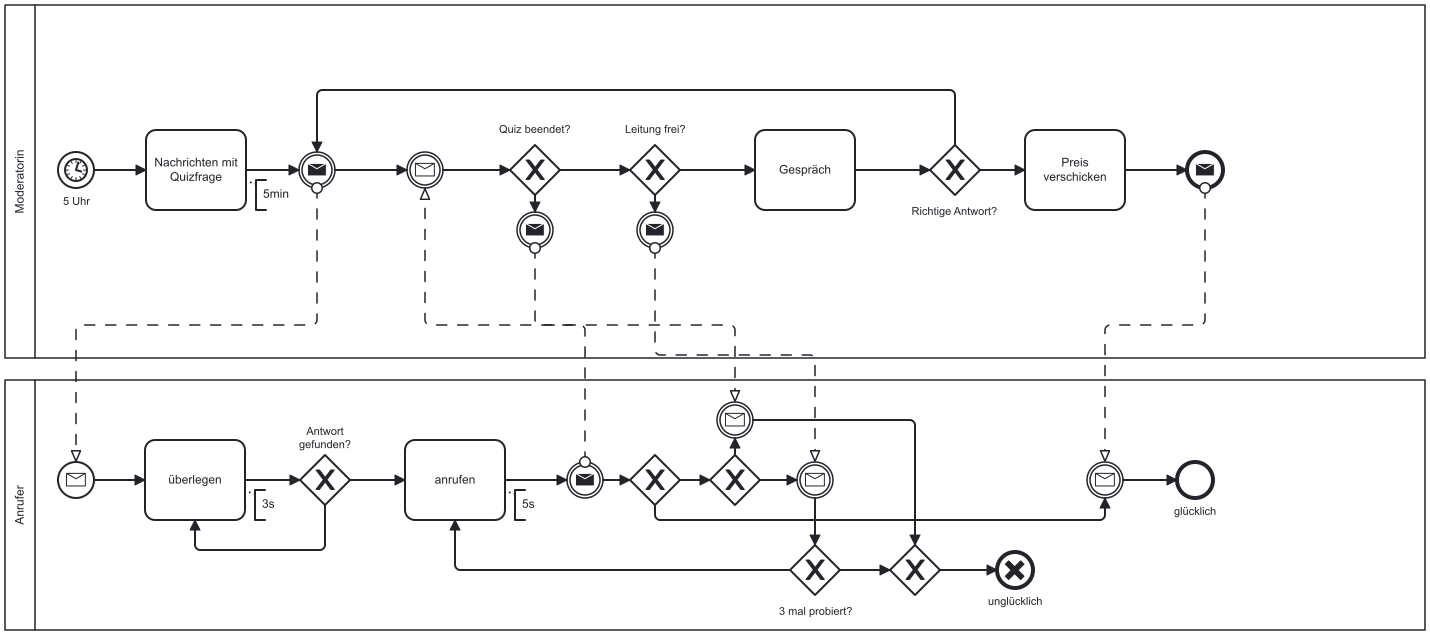
\includegraphics{res/bpmn-mock.png}
  }
  \caption{Modellierung des Quizzes}
\end{figure}
          \end{solution}
  \end{enumerate}

  \hint{
    \begin{itemize}
      \item Berücksichtigen Sie immer weitere Anrufe im Zeitverlauf, bis das Quiz beendet ist.
      \item Kennzeichnen Sie Verteilungen für die Dauer zeitkonsumierender Aktivitäten und die Länge von Zwischenankunftszeiten, eventuell benötigte Ressourcen sowie möglicherweise erforderliche Definitionen und Änderungen der Werte von prozesslokalen Attributen sowie globalen Variablen wie in der MuS-Vorlesung und -Übung durch Kommentare.
      \item BPMN-Start-/Zwischen-/Endereignisse können Sie in dieser Klausur mangels farbiger Stifte nicht in grün, gelb oder rot ausmalen. Verwenden Sie aber unbedingt, wie in BPMN üblich, eine einfache/dünne Umrandung für ein Startereignis, eine doppelte/dünne Umrandung für ein Zwischenereignis und eine einfache/dicke Umrandung für ein Endereignis.
      \item Verwenden Sie außerdem, wo immer dies sinnvoll ist, möglichst konkrete Typen von BPMN-Ereignissen, also z.B. Zeitsteuerung oder Nachrichtenereignisse statt allgemeinen ("unausgefüllten") Ereignissen.
      \item Wo die Modellbeschreibung nicht ausreichend präzise oder unvollständig ist, dürfen sinnvolle Annahmen getroffen werden. Nicht explizit in der Modellbeschreibung mit einer bestimmten Dauer erwähnte Aktivitäten dürfen als zeitverzugslos angenommen werden.
      \item Vergleichen Sie nach Abschluss der Aufgabe Ihre Antworten zu \ref{itm:ent2} und \ref{itm:mod2}. Insbesondere: Falls Sie während der Bearbeitung von \ref{itm:mod2} Korrekturbedarf bezüglich in der \ref{itm:ent2} benannten Entitäten, Ereignistypen oder Warteschlangen festgestellt haben, dann ändern Sie auch Ihre Antwort von \ref{itm:ent2} entsprechend!
    \end{itemize}
  }
\end{exercise}

\sheet[2023]{Altklausur}
\begin{exercise}{Modellierung}
  Gegeben sei folgenden Modellbeschreibung: Wir betrachten ein Stadion, welches Fußballspiele austrägt. Dies bringt logistische Herausforderungen mit sich:
  \par Die Fans nehmen die S-Bahn vom Hauptbahnhof zum Bahnhof in der Nähe des Stadions. Alle 5 Minuten verlässt eine S-Bahn den Hauptbahnhof mit 300-500 Fans (gleichverteilt). Die Fahrtzeit ist normalverteilt mit 15 Minuten Mittelwert und 2 Minuten Standardabweichung.
  \par Angekommen am Bahnhof steigen konstant 10 Fans pro Sekunde aus.
  \par Es wird ein Shuttle-Bus zum Stadion angeboten. Um diesen zu erreichen müssen die Fans einen Tunnel durchqueren. Es kann sich eine Warteschlange bilden, da der Tunnel nur eine begrenzte Anzahl von Fans durchlassen kann. Die Wartezeit ist exponentialverteilt mit einem Mittelwert von 5 Minuten.
  \par Der Bus fährt alle 100 Sekunden ab und kann beliebig viele Fans aufnehmen.
  \par Wenn das Warten länger als die individuelle Toleranz dauert (Mittelwert 300 Sekunden, exponentialverteilt), brechen die Fans das Warten ab und gehen zu Fuß zum Stadion.

  Bearbeiten Sie hierzu folgende Teilaufgaben.
  \begin{enumerate}
    \item Nennen Sie drei Leistungsgrößen die bei einer Simulation dieses Modells analysiert werden könnten.
          \begin{solution}
            \begin{enumerate}
              \item Die durchschnittliche Wartezeit der Fans im Tunnel.
              \item Die Anzahl der Fans, die den Shuttle-Bus nutzen.
              \item Die Anzahl der Fans, die zu Fuß zum Stadion gehen.
            \end{enumerate}
          \end{solution}
    \item\label{itm:empf3} Würden Sie eine ereignisorientierte oder eine prozessorientierte Modellierung vorschlagen?
          \begin{solution}
            \begin{enumerate}
              \item Ereignisorientierte Modellierung: Die Prozesse im Modell sind durch diskrete Ereignisse (Abfahrt der S-Bahn, Ankunft der Fans am Bahnhof, Warten im Tunnel, Abfahrt des Busses) gekennzeichnet.
              \item Ereignisorientierte Modelle sind besonders geeignet, um Systeme zu simulieren, bei denen sich der Zustand nur bei bestimmten, klar definierten Ereignissen ändert, was hier der Fall ist.
            \end{enumerate}
          \end{solution}
    \item\label{itm:ent3} Nennen Sie die Entitäten und teilen Sie diese in Prozesse \& Ressourcen ein.
          \begin{solution}
            \begin{enumerate}
              \item Entitäten:
                    \begin{enumerate}
                      \item Fans
                      \item S-Bahn
                      \item Bahnhof
                      \item Shuttle-Bus
                      \item Tunnel
                    \end{enumerate}
              \item Prozesse:
                    \begin{enumerate}
                      \item Abfahrt der S-Bahn
                      \item Ankunft der Fans am Bahnhof
                      \item Warten im Tunnel
                      \item Abfahrt des Busses
                    \end{enumerate}
              \item Ressourcen:
                    \begin{enumerate}
                      \item Tunnel
                    \end{enumerate}
            \end{enumerate}
          \end{solution}
    \item Unabhängig vom Ergebnis aus \ref{itm:empf3} soll eine prozessorientierte Modellierung mittels BPMN erfolgen. Prozessarten aus \ref{itm:ent3} modellieren.
          \begin{solution}
            % TODO: add BPMN diagram
          \end{solution}
  \end{enumerate}
\end{exercise}

\begin{exercise}{Mathematischer Themenblock}
  \begin{enumerate}
    \item Beschreiben Sie kurz den Zentralen Grenzwertsatz und nennen Sie eine Anwendung.
          \begin{solution}
            Der Zentrale Grenzwertsatz besagt, dass die Summe von unabhängigen, identisch verteilten Zufallsvariablen einer beliebigen Verteilung für eine große Anzahl von Summanden annähernd normalverteilt ist. Eine Anwendung ist die Schätzung von Mittelwerten in Stichproben.
          \end{solution}
    \item Wie läuft eine ereignisbasierte Simulation ab? Was ist in diesen Kontext eine Ereignisliste?
          \begin{solution}
            Bei einer ereignisbasierten Simulation werden diskrete Ereignisse in einem System modelliert und simuliert. Die Simulation beginnt mit der Initialisierung des Systems und der Erzeugung des ersten Ereignisses. Die Ereignisse werden in einer Ereignisliste gespeichert und nach ihrer Zeitstempel-Reihenfolge abgearbeitet.
          \end{solution}
    \item Unterscheiden Sie ereignis- \& zeitintervallbasierte Simulation!
          \begin{solution}
            Ereignisbasierte Simulation: Simulation basierend auf diskreten Ereignissen, die den Zustand des Systems verändern. Zeitintervallbasierte Simulation: Simulation basierend auf kontinuierlichen Zeitintervallen, die den Zustand des Systems beschreiben.
          \end{solution}
  \end{enumerate}
\end{exercise}

\begin{exercise}{Qualitative \& Quantitative Prozessanalysetechniken}
  \begin{enumerate}
    \item Nennen Sie jeweils zwei qualitative und zwei quantitative Prozessanalysetechniken und beschreiben Sie diese kurz.
          \begin{solution}
            Qualitative Prozessanalysetechniken sind zum Beispiel Interviews und Workshops. Quantitative Prozessanalysetechniken sind zum Beispiel Prozesssimulation und Prozessmining.
            In Interviews werden Mitarbeiter befragt, um Informationen über Prozesse zu sammeln. In Workshops werden Mitarbeiter in Gruppen zusammengebracht, um Prozesse zu analysieren und zu verbessern.
            Prozesssimulation ist die Nachbildung von Prozessen in einem Modell, um deren Verhalten zu analysieren. Prozessmining ist die Analyse von Prozessdaten zur Identifikation, Überwachung und Verbesserung von Geschäftsprozessen.
          \end{solution}
    \item Wie kann man die Critical Task Execution optimieren?
          \begin{solution}
            Die Critical Task Execution kann durch die Identifikation und Priorisierung kritischer Aufgaben, die Automatisierung von Routineaufgaben und die Verbesserung der Kommunikation und Zusammenarbeit zwischen Mitarbeitern optimiert werden.
          \end{solution}
  \end{enumerate}
\end{exercise}

\begin{exercise}{BPMN}
  \begin{enumerate}
    \item Nennen Sie zwei Nachteile von BPMN und beschreiben Sie diese kurz.
          \begin{solution}
            Nachteile von BPMN sind zum Beispiel die Komplexität und die Abstraktion. Komplexität: BPMN-Diagramme können sehr komplex werden und sind schwer zu verstehen. Abstraktion: BPMN-Diagramme sind abstrakt und können von Mitarbeitern falsch interpretiert werden.
          \end{solution}
    \item Was ist Process Mining und wie kann man den Nachteilen von BPMN mithilfe von Process Mining entgegenwirken?
          \begin{solution}
            Process Mining ist die Analyse von Prozessdaten zur Identifikation, Überwachung und Verbesserung von Geschäftsprozessen. Process Mining kann dazu beitragen, die Nachteile von BPMN zu überwinden, indem es die tatsächliche Ausführung von Prozessen analysiert und Verbesserungspotenziale aufdeckt.
          \end{solution}
  \end{enumerate}
\end{exercise}

\begin{exercise}{ERP-Systeme}
  \begin{enumerate}
    \item Würden Sie McDongerKing eine ERP-Standardsoftware oder Individualsoftware empfehlen? Begründen Sie Ihre Antwort.
          \begin{solution}
            Da McDongerKing mehrere Filialen betreibt und ein Online-Bestell-System unterhält, allerdings wahrscheinlich nicht die Ressourcen für die Entwicklung einer Individualsoftware hat, würde ich McDongerKing eine ERP-Standardsoftware empfehlen.
          \end{solution}
    \item Wäre eine ERP-Cloud Lösung sinnvoll?
          \begin{solution}
            Eine ERP-Cloud Lösung könnte für McDongerKing sinnvoll sein, da sie flexibel und skalierbar ist und keine hohen Investitionskosten erfordert.
          \end{solution}
  \end{enumerate}
\end{exercise}

\begin{exercise}{IT-Governance}
  Nennen Sie zwei Aufgaben der IT-Governance und beschreiben Sie diese kurz.

  \begin{solution}
    IT-Strategie: Entwicklung und Umsetzung einer IT-Strategie, IT-Compliance: Sicherstellung der Einhaltung von gesetzlichen und regulatorischen Anforderungen.
  \end{solution}
\end{exercise}

\begin{exercise}{IT-Strategie \& Digital Business Strategie}
  Erklären Sie den Unterschied zwischen IT-Strategie und Digital Business Strategie anhand von drei charakteristischen Eigenschaften der beiden und nennen Sie Beispiele.

  \begin{solution}
    Wichtige Unterschiede zwischen IT-Strategie und Digital Business Strategie sind: Fokus, Umfang und Ziele. IT-Strategie: Fokus auf IT-Infrastruktur und -Systeme, Umfang begrenzt auf IT-Systeme, Ziele sind Effizienz und Effektivität. Digital Business Strategie: Fokus auf digitale Technologien und Geschäftsmodelle, Umfang umfasst das gesamte Unternehmen, Ziele sind Wettbewerbsvorteile und Innovation.
  \end{solution}
\end{exercise}

\begin{exercise}{Soziotechnische Systeme}
  Nennen Sie zwei Prinzipien der Entwicklung soziotechnischer Systeme und beschreiben Sie diese kurz.

  \begin{solution}
    Partizipation: Einbeziehung der Mitarbeiter in den Entwicklungsprozess, Transparenz: Offenlegung von Entscheidungen und Prozessen.
  \end{solution}
\end{exercise}


\sheet[2022]{Altklausur}

\begin{exercise}{Ereignisorientierte Modellierung}
  Nennen Sie vier typische Zwecke, warum man lieber an Modellen Untersuchungen durchführt, statt am Realsystem und je ein Beispiel nennen.
  \begin{solution}
    \begin{enumerate}
      \item Kostenersparnis: Simulation eines Flughafens, um die Anzahl der benötigten Sicherheitskontrollen zu bestimmen.
      \item Risikominimierung: Simulation eines Produktionsprozesses, um Engpässe zu identifizieren.
      \item Effizienzsteigerung: Simulation eines Logistiksystems, um die optimale Routenplanung zu bestimmen.
      \item Komplexität: Simulation eines Finanzsystems, um die Auswirkungen von Änderungen zu analysieren.
    \end{enumerate}
  \end{solution}

  Ereignisorientierte Modellierung analog zur Probeklausur.
\end{exercise}

\begin{exercise}{Systemmodellierung}
  \begin{enumerate}
    \item Nennen Sie einen Vorteil und einen Nachteil für Systemmodellierung auf der Werkzeugebene und beschreiben Sie diese.
          \begin{solution}
            Vorteil einer Systemmodellierung auf der Werkzeugebene ist Strukturierung: Systemmodellierung hilft, komplexe Systeme zu strukturieren und zu visualisieren. Nachteil einer Systemmodellierung auf der Werkzeugebene ist Vereinfachung: Systemmodelle sind abstrakt und können die Realität vereinfachen.
          \end{solution}
    \item Beschreiben Sie das "Zwischenereignis mit empfangener Nachricht".
          \begin{solution}
            Ein Zwischenereignis mit empfangener Nachricht ist ein Ereignis, das auftritt, wenn eine Nachricht empfangen wird.
          \end{solution}
  \end{enumerate}
\end{exercise}

\begin{exercise}{Anlauf von Simulationen}
  Wann ist eine Simulation fertig "angelaufen"?

  \begin{solution}
    Eine Simulation ist fertig "angelaufen", wenn die Initialisierung abgeschlossen ist und die Simulation gestartet wurde.
  \end{solution}
\end{exercise}

\begin{exercise}{Teile von Organisationen}
  \begin{enumerate}
    \item Nennen Sie die fünf Teile einer Organisation und beschreiben Sie diese kurz.
          \begin{solution}
            % TODO: add
          \end{solution}
    \item Ordnen Sie McDongerKing in ein Organisationsdesign ein und begründen Sie dies mit Mechanismen, Koordination und Intention.
          \begin{solution}
            % TODO: add
          \end{solution}
  \end{enumerate}
\end{exercise}

\begin{exercise}{McDongerKing}
  Was muss man beachten, wenn McDongerKing DIU (Digitale Innovationseinheiten) einführen will?

  \begin{solution}
    Bei der Einführung von DIU muss McDongerKing darauf achten, dass die DIU in die bestehende Organisation integriert werden und die Mitarbeiter in den Entwicklungsprozess einbezogen werden.
  \end{solution}
\end{exercise}

\begin{exercise}{Digital Business Strategy}
  Definieren Sie Digital Business Strategy (DBS).

  \begin{solution}
    Digital Business Strategy (DBS) ist die Entwicklung und Umsetzung einer Strategie, um digitale Technologien und Geschäftsmodelle zu nutzen, um Wettbewerbsvorteile zu erzielen.
  \end{solution}
\end{exercise}

\end{document}